\documentclass[12pt,A4]{article}
\usepackage[dvipsnames,rgb,dvips]{xcolor}
\usepackage{graphicx}
\usepackage{psfrag}
\usepackage{dcolumn}
\usepackage{bm}
\usepackage{amsmath}
\usepackage{amssymb}
\usepackage[rflt]{floatflt}
\usepackage{latexsym}
\addtolength{\topmargin}{-1.9cm}
\addtolength{\textheight}{5.5cm}
\addtolength{\evensidemargin}{-1.2cm}
\addtolength{\oddsidemargin}{-1.2cm}
\addtolength{\textwidth}{2cm}
\pagestyle{myheadings}
\markright{{\small Edin Citaku \hfill (XXYYZZ-ABCD) \,}}
\begin{document}
\parindent=0cm

\begin{figure}
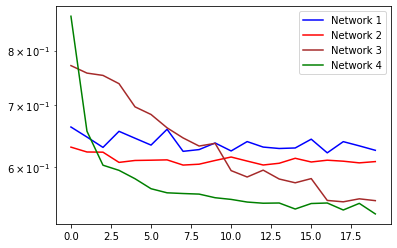
\includegraphics[scale=1]{hw3-1-graph.png}
\begin{center}
\end{center}
\caption{Classification error for each network as a graph of epochs\label{fig}}
\end{figure}
It is clear that the addition of a second layer improves the learning performance significant, while adding neurons to a layer did not show a big boost in performance for the case of a hidden layer size of 1 and 2.
The classification error of the test set is slightly less than of the validation set, pointing to the possibility of overfitting.
Training set shows a classification error of 9.0, pointing to a bug in the code. Here it would be expected, that the classification error is the lowest.
The data shows, that added complexity does not necessarily result in improved performance. Furthermore it shows that it is easy to overfit a network and one should be vary when analyzing their results.
\begin{figure}
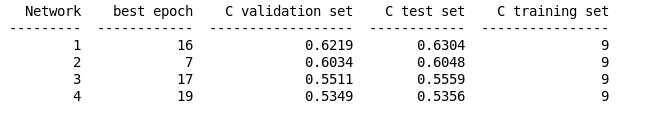
\includegraphics[scale=0.7]{hw3-1-table.png}
\begin{center}
\end{center}
\caption{table with the classification error\label{tab}}
\end{figure}
\end{document}
